\documentclass[aspectratio=169]{beamer}
\usepackage[T1]{fontenc}
\usepackage[utf8]{inputenc}
\usepackage{lmodern}
\usepackage{microtype}
\usepackage{xcolor}
\usepackage{tikz}
\usetikzlibrary{positioning, arrows.meta, calc}
\usepackage{fontawesome5}
\definecolor{wurgreen}{HTML}{34B233}
\definecolor{darkgreen}{HTML}{1F6B1E}
\definecolor{darknavy}{HTML}{1A1A2E}
\definecolor{midgray}{HTML}{6B7280}
\definecolor{lightgray}{HTML}{F3F4F6}
\definecolor{lightgreen}{HTML}{E8F7E8}
\definecolor{bodytext}{HTML}{1F2937}
\definecolor{warnred}{HTML}{FEE2E2}
\definecolor{warnborder}{HTML}{EF4444}
\definecolor{codebg}{HTML}{1E1E2E}
\definecolor{codegreen}{HTML}{9ECE6A}
\definecolor{codeblue}{HTML}{7AA2F7}
\definecolor{codeorange}{HTML}{FF9E64}
\definecolor{codegray}{HTML}{C0CAF5}
\usetheme{default}\usecolortheme{default}\usefonttheme{professionalfonts}
\setbeamertemplate{navigation symbols}{}
\setbeamertemplate{itemize items}{\textcolor{wurgreen}{\textbullet}}
\setbeamertemplate{itemize subitem}{\textcolor{midgray}{--}}
\setbeamercolor{frametitle}{fg=white, bg=darknavy}
\setbeamerfont{frametitle}{size=\large, series=\bfseries}
\setbeamertemplate{frametitle}{%
  \begin{beamercolorbox}[wd=\paperwidth, ht=1.1cm, dp=0.2cm, leftskip=0.6cm]{frametitle}
    \usebeamerfont{frametitle}\insertframetitle\end{beamercolorbox}}
\setbeamercolor{background canvas}{bg=white}
\setbeamercolor{normal text}{fg=bodytext}
\setbeamertemplate{footline}{%
  \begin{beamercolorbox}[wd=\paperwidth, ht=0.4cm, dp=0.15cm]{footline}
    \hspace{0.5cm}\textcolor{midgray}{\tiny Introduction to Python · Module 7: pandas}%
    \hfill\textcolor{midgray}{\tiny \insertframenumber}\hspace{0.4cm}\end{beamercolorbox}}
\newcommand{\codebox}[1]{\begin{center}
  \begin{tikzpicture}\node[fill=codebg, rounded corners=4pt, inner sep=9pt, text width=0.85\textwidth, text=codegray]{\ttfamily\small #1};\end{tikzpicture}\end{center}}
\begin{document}
{\setbeamertemplate{footline}{}
\begin{frame}[plain]
  \begin{tikzpicture}[remember picture, overlay]
    \fill[darknavy] (current page.south west) rectangle (current page.north east);
    \fill[wurgreen] (current page.south west) rectangle ([xshift=0.45cm]current page.north west);
    \node[anchor=west, text=white, font=\huge\bfseries, text width=13cm] at ([xshift=1.1cm, yshift=1.4cm]current page.west){Introduction to Python};
    \node[anchor=west, text=wurgreen, font=\large, text width=12cm] at ([xshift=1.1cm, yshift=0.2cm]current page.west){Module 7 --- pandas};
    \node[anchor=west, text=midgray, font=\small, text width=12cm] at ([xshift=1.1cm, yshift=-1.3cm]current page.west){DataFrames, filtering, grouping, and plotting};
  \end{tikzpicture}
\end{frame}}

\begin{frame}{What Is Pandas?}
\vspace{0.2cm}
{\small \textbf{pandas} is \emph{the} library for working with data tables in Python --- think of
it as a programmable spreadsheet. Its core object is the \textbf{DataFrame}: rows and columns,
like an Excel sheet.}
\medskip
\codebox{%
\textcolor{codeblue}{import} pandas \textcolor{codeblue}{as} pd\\[6pt]
df \textcolor{codegray}{=} pd.\textcolor{codeblue}{DataFrame}(\{\\
\quad\textcolor{codegreen}{"city"}: [\textcolor{codegreen}{"Wageningen"}, \textcolor{codegreen}{"Utrecht"}],\\
\quad\textcolor{codegreen}{"population"}: [\textcolor{codeorange}{40000}, \textcolor{codeorange}{360000}]\\
\})}
\medskip
{\small \texttt{import pandas as pd} is the universal convention. A DataFrame has \textbf{named
columns} and \textbf{indexed rows} --- and hundreds of methods for slicing, filtering, and
summarizing.}
\end{frame}

\begin{frame}{Loading Real Data}
\vspace{0.2cm}
{\small Most of the time you don't type data by hand --- you \textbf{load a file}. pandas reads
CSVs (and Excel, JSON, and more) in one line.}
\medskip
\codebox{%
df \textcolor{codegray}{=} pd.\textcolor{codeblue}{read\_csv}(\textcolor{codegreen}{"data.csv"})\\[8pt]
df.\textcolor{codeblue}{head}()\quad\ \ \ \ \textcolor{codegray}{\# first 5 rows}\\
df.\textcolor{codeblue}{shape}\quad\ \ \ \ \ \textcolor{codegray}{\# (rows, columns)}\\
df.\textcolor{codeblue}{columns}\quad\ \ \ \textcolor{codegray}{\# the column names}\\
df.\textcolor{codeblue}{info}()\quad\ \ \ \ \textcolor{codegray}{\# types \& missing values}\\
df.\textcolor{codeblue}{describe}()\quad\ \textcolor{codegray}{\# summary statistics}}
\medskip
{\small\textcolor{midgray}{\textit{\texttt{head()}, \texttt{info()}, and \texttt{describe()} are
the first three things you run on any new dataset --- always look before you leap.}}}
\end{frame}

\begin{frame}{Selecting Columns \& Rows}
\vspace{0.2cm}
\codebox{%
\textcolor{codegray}{\# a single column (by name)}\\
df[\textcolor{codegreen}{"population"}]\\[6pt]
\textcolor{codegray}{\# several columns}\\
df[[\textcolor{codegreen}{"city"}, \textcolor{codegreen}{"population"}]]\\[6pt]
\textcolor{codegray}{\# rows by position with .iloc}\\
df.\textcolor{codeblue}{iloc}[\textcolor{codeorange}{0}]\quad\ \ \ \textcolor{codegray}{\# the first row}\\
df.\textcolor{codeblue}{iloc}[\textcolor{codeorange}{0}:\textcolor{codeorange}{3}]\quad\ \textcolor{codegray}{\# the first three rows}}
\medskip
{\small A single column is called a \textbf{Series}. Selecting columns uses their \textbf{names};
selecting rows by position uses \texttt{.iloc}. (There's also \texttt{.loc} for selecting by
label.)}
\end{frame}

\begin{frame}{Filtering Rows by Condition}
\vspace{0.2cm}
{\small The most common data task: keep only the rows that meet a condition. pandas uses the same
boolean idea as NumPy.}
\medskip
\codebox{%
\textcolor{codegray}{\# cities with more than 100,000 people}\\
big \textcolor{codegray}{=} df[df[\textcolor{codegreen}{"population"}] \textcolor{codegray}{>} \textcolor{codeorange}{100000}]\\[8pt]
\textcolor{codegray}{\# combine conditions with \& (and), | (or)}\\
df[(df[\textcolor{codegreen}{"population"}] \textcolor{codegray}{>} \textcolor{codeorange}{50000}) \textcolor{codegray}{\&}\\
\quad\ \ (df[\textcolor{codegreen}{"city"}] \textcolor{codegray}{!=} \textcolor{codegreen}{"Utrecht"})]}
\medskip
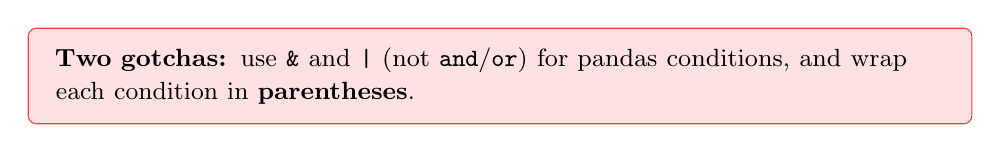
\begin{tikzpicture}
  \node[fill=warnred, draw=warnborder, rounded corners=3pt, inner xsep=10pt, inner ysep=7pt, text width=\textwidth-24pt]{%
    {\small \textbf{Two gotchas:} use \texttt{\&} and \texttt{|} (not \texttt{and}/\texttt{or})
    for pandas conditions, and wrap each condition in \textbf{parentheses}.}};
\end{tikzpicture}
\end{frame}

\begin{frame}{New Columns \& Grouping}
\vspace{0.2cm}
{\small Two everyday operations: \textbf{creating columns} and \textbf{grouping} to summarize.}
\medskip
\codebox{%
\textcolor{codegray}{\# create a new column from existing ones}\\
df[\textcolor{codegreen}{"pop\_thousands"}] \textcolor{codegray}{=} df[\textcolor{codegreen}{"population"}] \textcolor{codegray}{/} \textcolor{codeorange}{1000}\\[8pt]
\textcolor{codegray}{\# group and summarize: mean population per region}\\
df.\textcolor{codeblue}{groupby}(\textcolor{codegreen}{"region"})[\textcolor{codegreen}{"population"}].\textcolor{codeblue}{mean}()}
\medskip
{\small \texttt{groupby} is the powerhouse of data analysis: split the data into groups, compute
something per group (\texttt{mean}, \texttt{sum}, \texttt{count}\ldots), and combine the results.
It answers ``what's the average X for each Y?''}
\end{frame}

\begin{frame}{Quick Plots from a DataFrame}
\vspace{0.2cm}
{\small pandas has plotting built in --- one method, and you get a chart (it uses matplotlib
underneath).}
\medskip
\codebox{%
\textcolor{codegray}{\# a bar chart of population by city}\\
df.\textcolor{codeblue}{plot}(x\textcolor{codegray}{=}\textcolor{codegreen}{"city"}, y\textcolor{codegray}{=}\textcolor{codegreen}{"population"}, kind\textcolor{codegray}{=}\textcolor{codegreen}{"bar"})\\[8pt]
\textcolor{codegray}{\# a histogram of a numeric column}\\
df[\textcolor{codegreen}{"population"}].\textcolor{codeblue}{plot}(kind\textcolor{codegray}{=}\textcolor{codegreen}{"hist"})}
\medskip
{\small\textcolor{midgray}{\textit{\texttt{kind} can be \texttt{"bar"}, \texttt{"line"},
\texttt{"hist"}, \texttt{"scatter"}, and more. Great for a quick look; for polished figures you'd
use matplotlib or seaborn directly.}}}
\end{frame}

\begin{frame}{Module 7: Takeaways}
\vspace{0.3cm}
\begin{itemize}\setlength\itemsep{7pt}
  \item[\textcolor{wurgreen}{\faCheck}] \texttt{import pandas as pd}; the \textbf{DataFrame} is a programmable table
  \item[\textcolor{wurgreen}{\faCheck}] \texttt{pd.read\_csv()} loads data; \texttt{head() info() describe()} explore it
  \item[\textcolor{wurgreen}{\faCheck}] Select columns by \textbf{name}, rows by position with \texttt{.iloc}
  \item[\textcolor{wurgreen}{\faCheck}] \textbf{Filter} with boolean conditions (use \texttt{\&} \texttt{|} and parentheses)
  \item[\textcolor{wurgreen}{\faCheck}] Create columns, and \texttt{groupby()} to summarize per group
  \item[\textcolor{wurgreen}{\faCheck}] \texttt{.plot()} gives quick charts straight from the DataFrame
\end{itemize}
\medskip
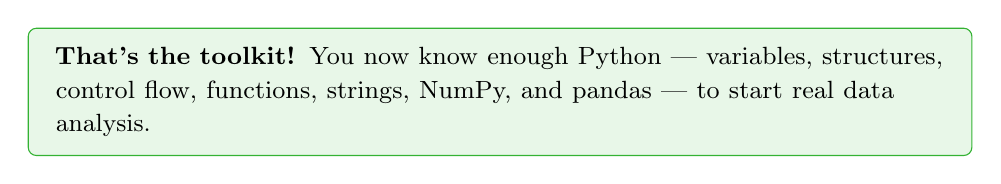
\begin{tikzpicture}
  \node[fill=lightgreen, draw=wurgreen, rounded corners=3pt, inner xsep=10pt, inner ysep=7pt, text width=\textwidth-24pt]{%
    {\small \textbf{That's the toolkit!} You now know enough Python --- variables, structures,
    control flow, functions, strings, NumPy, and pandas --- to start real data analysis.}};
\end{tikzpicture}
\end{frame}
\end{document}
